\section{Vehicle Counter}
\label{sec:system-counter}

In collaboration with \gls{idot}, we want to have the vehicle counting statistics as the final results. To get the  vehicle counts along different motions, we also need to know the motions available in each video. 

\subsection{Vehicle Counter with Human Annotation}
Initially, we build a GUI interface and ask the user to draw a few line segments to indicate a motion template. \ref{fig:anno-gui} is the screen shot of the interface, where the motion templates mostly align with the road surface but may have more than one for each road. 
\ref{fig:kf-counter} shows our first counter framework without semantic knowledge. The vehicle tracker will generate a set of vehicle trajectories, by assigning each trajectory to a motion template and increase the corresponding count, we can obtain the final traffic count. 

Suppose we have a set of $n$ motion templates $\mathbf{T} = \{\mathbf{T}_1, \mathbf{T}_2, \dots, \mathbf{T}_n\}$ and a set of trajectories of $N$ vehicles $\Omega= \{\mathbf{O}_1, \mathbf{O}_2, \dots, \mathbf{O}_N\}$.

\begin{figure}
\centering
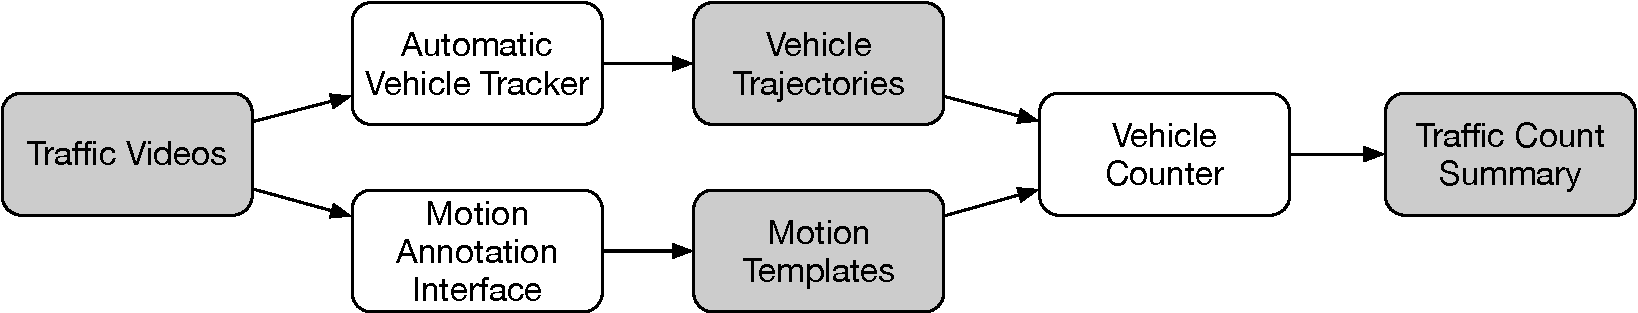
\includegraphics[width=\linewidth]{./img/system/kf-counter.pdf}
\caption{Vehicle counter workflow with human annotation.}
\label{fig:kf-counter}
\end{figure}
\begin{figure}
\centering
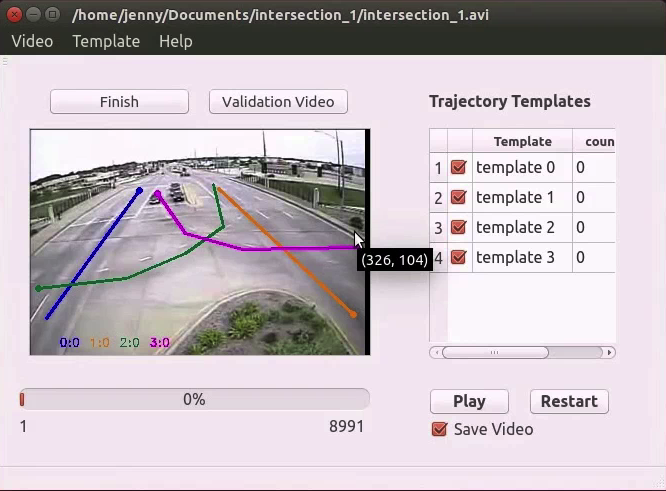
\includegraphics[width=\linewidth]{./img/system/line_seg.png}
\caption{Motion annotation interface.}
\label{fig:anno-gui}
\end{figure}

\subsection{Vehicle Counter with Semantic Knowledge}
With offline learned semantic knowledge per camera, the system becomes end-to-end without any human input. 
\ref{fig:semantic-counter} shows the workflow of the improved counter with semantic knowledge. 
Motion topics are learned fully automatically.
By online inference, each tracked vehicle is assigned to a motion until leaving, therefore, the counting is finished along tracking. 

\begin{figure}
\centering
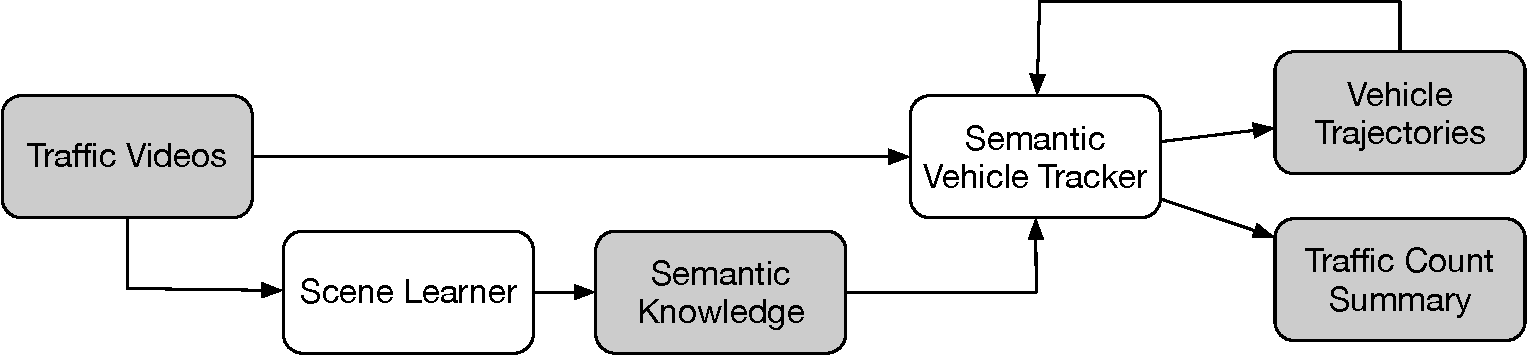
\includegraphics[width=\linewidth]{./img/system/semantic-counter.pdf}
\caption{End-to-end vehicle counter workflow with scene understanding.}
\label{fig:semantic-counter}
\end{figure}

\subsection{Web Portal}
For remote access, we build a web portal for this system for \gls{idot}. Currently the scene understanding module has not been integrated, only the what shown in \ref{fig:kf-counter} is implemented.
Cameras are displayed on map as shown in \ref{fig:sys-main}, with a list of their name on the left. Users may create or browse cameras by list or map, and upload videos for each camera. Once a new camera is created and the first video is uploaded, the user need to draw the motion templates.
Once a video is uploaded, the tracker and counter will be called in the background. Users may return later to check and download the results. We allow at most four videos processed at the same time. 
\ref{fig:sys-camera} and \ref{fig:sys-video} are the camera view and video view with traffic summary and visualization. 
Each camera may have multiple videos. Summary of all the videos is displayed. In the video view, counts of different motions are displayed.
\begin{figure}
    \centering
    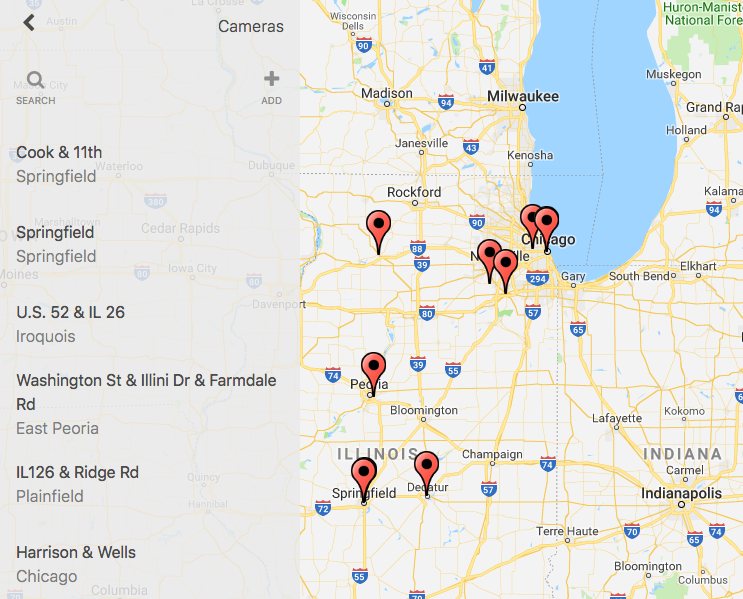
\includegraphics[width=\linewidth]{./img/system/main.png}
    \caption{Main interface of the web portal, cameras are displayed on the map.}
    \label{fig:sys-main}
\end{figure}
\begin{figure}
    \centering
    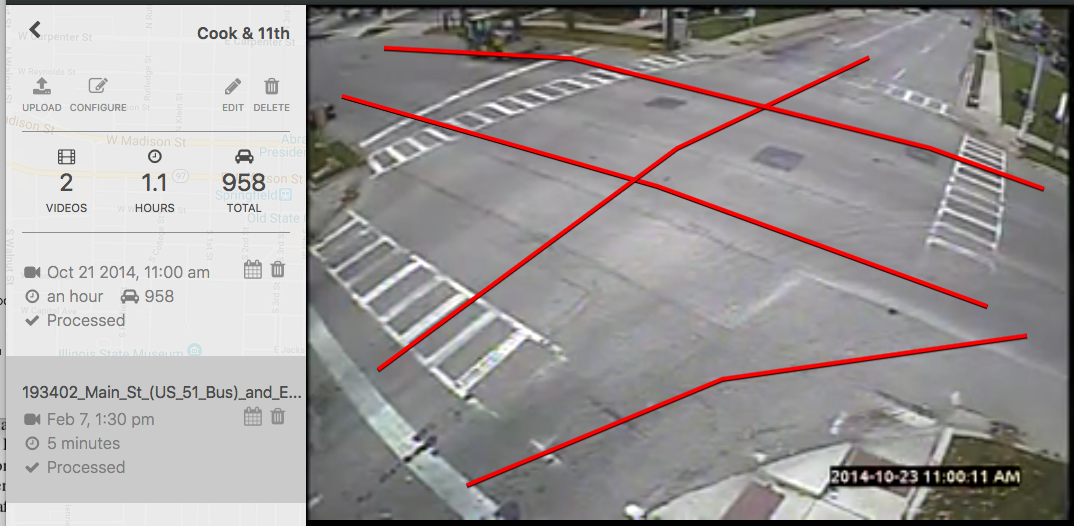
\includegraphics[width=\linewidth]{./img/system/camera.png}
    \caption{Camera view with video list and summary.}
    \label{fig:sys-camera}
\end{figure}
\begin{figure}
    \centering
    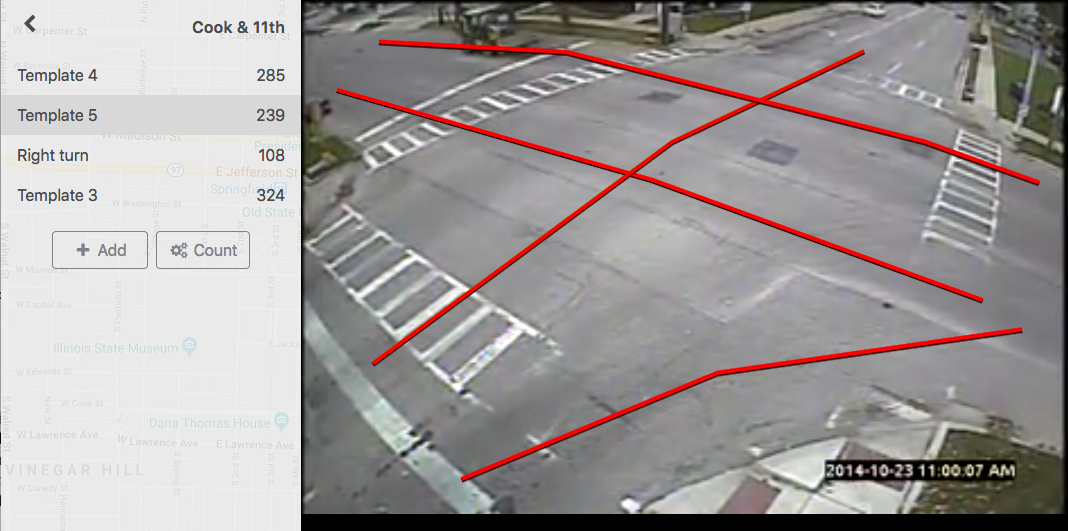
\includegraphics[width=\linewidth]{./img/system/video.png}
    \caption{Individual video view with counting information.}
    \label{fig:sys-video}
\end{figure}
